\chapter{Hierarchical Clustering}


\section{Learning Objectives}

\begin{itemize}

\item Understand hierarchical clustering algorithm

\item Implement the algorithm
  
\item Learn the binary tree and its properties

\item Use the tree's properties to gain insight of data
  
\end{itemize}

\section{Limitations of the {\it k-mean} Algorithm}

The {\it k-mean} clustering algorithm has several major problems:
\begin{enumerate}
  \item 
There is no obvious reason to select a particular value of $k$.
Figure~\ref{figure:kmean:distances} shows the distances for different
values of $k$. There are 10 clusters and the clusters do not overlap
({\tt -t} not used) but the smallest distance occurs when $k$ is 13.

\item The algorithm is non-deterministic and it is often necessary
  running the same program multiple times.
  Figure~\ref{figure:kmean:distances} (a) shows that the distances may
  vary substantially even for the same value of $k$.

\item For a given cluster, there is no easy answer which cluster is
  closer.  It is possible to calculate the distances of centroids but
  this requires additional work.

\item The {\it k-mean} algorithm assigns {\it all} data points to one
  of the $k$ clusters in the very first step.  Then the algorithm
  adjusts the clusters by the finding closest centroid from each data
  point. Because the initial assignments have direct impacts on the
  final results, the program needs to run multiple times for getter
  better results.  
\end{enumerate}

\index{binary tree}
\index{binary tree!child}

{\it Hierarchical clustering} is a method that does
  not have these problems\footnote{Hierarchical clustering has some
    other problems, to be discussed later.}.

\section{Example of 
Hierarchical clustering}

Hierarchical clustering iteratively finds the closest pair of data
points, clusters, or data point and cluster. The algorithm makes the
pair two {\it children} of a {\it binary tree}
node\marginnote{Hierarchical clustering calls it {\it dendrogram},
  instead of {\it binary tree}. This book uses both terms
  interchangably.}.  The tree node becomes a new cluster.  The
algorithm continues until only one tree node is left.

Before formally describing the algorithm, let us go through several
examples.  The simplest case is when there is only one data point but
it is not very meaningful. Thus, let us start with two data points.

\begin{table}[h]
\begin{tt}
\begin{tabular}{|r|rr|} \hline
{\bf index} &  {\bf x} & {\bf y} \\ \hline
0 &  -66  &  45 \\
1 & 95  &  -84 \\ \hline
\end{tabular}
\end{tt}
\end{table}

They are the two children of a binary tree:

\begin{figure}[h] \centering
{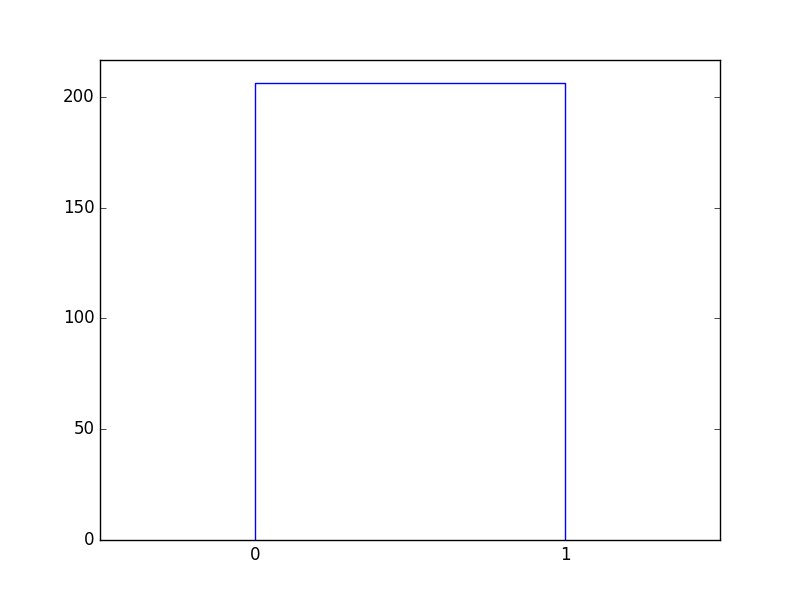
\includegraphics[width=5in]{\hierpath/figures/cluster2.png}}
\caption{Two data points are the two children of a binary tree. }
\label{fig:hierarchical:cluster2}
\end{figure}

Next, we consider the case when there are four data points:

\begin{table}[h]
\begin{tt}
\begin{tabular}{|r|rr|} \hline
{\bf index} &  {\bf x} & {\bf y} \\ \hline
0 &  -66  &  45 \\
1 & 95  &  -84 \\
2 & -35  &  -70 \\
3 & 26  &  94 \\ \hline
\end{tabular}
\end{tt}
\end{table}


Table~\ref{table:hierarchical:distance4points} shows the distance
between each pair of data points.  The distance of $(x_a, y_a)$ and
$(x_b, y_b)$ is $\sqrt{(x_a - x_b)^2 + (y_a - y_b)^2}$. Since we care
about the order, it is not necessary to take the square root.
The
table shows ${(x_a - x_b)^2 + (y_a - y_b)^2}$:
Obviously, this table is symmetric because the distance between $(x_a,
y_a)$ and $(x_b, y_b)$ is the same as distance between $(x_b, y_b)$
and $(x_a, y_a)$. The values along the diagnoal are always zero
because the distance of each point and itself is zero.

\begin{table}
  \begin{tt}
\begin{tabular}{|r|rrrr|}  \hline
& 0 & 1 & 2 & 3  \\ \hline

0 & 0& 42562& 14186& 10865\\
1 & 42562& 0& 17096& 36445\\
2 & 14186& 17096& 0& 30617\\
3 & 10865& 36445& 30617& 0\\ \hline
\end{tabular}
  \end{tt}
  \caption{Distances of pairs of data points.}
  \label{table:hierarchical:distance4points}
\end{table}

The shortest distance (10865) occurs between $(x_0, y_0)$ and $(x_3,
y_3)$.  They are the first pair to be put into the same cluster.
Figure~\ref{fig:hierarchical:cluster4} shows the cluster of the four
data points. Points 0 and 3 are the two children of the same parent
node.

\begin{figure}[h] \centering
{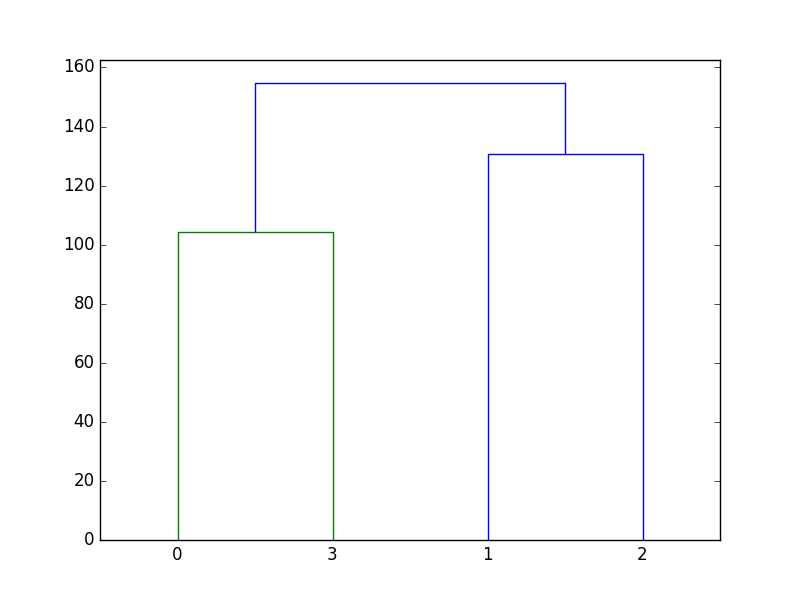
\includegraphics[width=5in]{\hierpath/figures/cluster4.png}}
\caption{Clusters of four data points.
Do not worry about the colors, nor the numbers along the vertical
axis. Pay attention to the shape only.
}
\label{fig:hierarchical:cluster4}
\end{figure}

How do we represent the cluster that includes points 0 and 3?  There
are several different commonly used representations.  This example
uses the {\it centroid}: a cluster is represented by the centroid of
the data points in the cluster. It is possible to represent a cluster
using other methods, to be discussed later in this chapter.  The
cluster that contains $(x_0, y_0)$ and $(x_3, y_3)$ is represented by
$(\frac{-66+26}{2}, \frac{45+94}{2}) = (-20, 69.5)$.  This cluster is
marked as the new $(x_0, y_0)$ and $(x_3, y_3)$ no longer exists.  We
can recompute the distances among the pairs of points:


\begin{table}
  \begin{tt}
\begin{tabular}{|r|rrr|}  \hline
& 0 & 1 & 2   \\ \hline

0 & 0.0 & 36787.25 & 19685.25 \\
1 & 36787.25 & 0 & 17096 \\
2 & 19685.25 & 17096 & 0 \\ \hline
\end{tabular}
  \end{tt}
  \caption{Distances of one cluster and two  data points.}
  \label{table:hierarchical:distance3}
\end{table}

Now, the shortest distance (17096) occurs between $(x_1, y_1)$ and
$(x_2, y_2)$.  These two data points are the two children of a tree
node.  At this moment, there are only two clusters and they are the
children of a binary tree node.  The final result is shown in
Figur~\ref{fig:hierarchical:cluster4}.

Let's add two more data points into consideration.

\begin{table}[h]
\begin{tt}
\begin{tabular}{|r|rr|} \hline
{\bf index} &  {\bf x} & {\bf y} \\ \hline
0 & -66 &  45 \\
1 & 95  &  -84 \\
2 & -35  &  -70 \\
3 & 26  &  94 \\
4 & 15 & 20 \\
5 & 66 & -3 \\ \hline
\end{tabular}
\end{tt}
\end{table}

The pair-wise distances is shown in
Table~\ref{table:hierarchical:distance6points}.

\begin{table}
  \begin{tt}
\begin{tabular}{|r|rrrrrr|}  \hline
& 0 & 1 & 2 & 3 & 4 & 5 \\ \hline

0 & 0& 42562& 14186& 10865 & 7186 & 19728\\
1 & 42562& 0& 17096& 36445 & 17216 & 7402\\
2 & 14186& 17096& 0& 30617 & 10600 & 14690\\
  3 & 10865& 36445& 30617& 0 & 5597 & 11009 \\
  4 & 7186 & 17216 & 10600 & 5597 & 0 & 3130 \\ 
  5 & 19728 & 7402 & 14690 & 11009 & 3130 & 0   \\ \hline
\end{tabular}
  \end{tt}
  \caption{Distances of pairs of six data points.}
  \label{table:hierarchical:distance6points}
\end{table}

The shortest distance (3130) occurs between $(x_4, y_4)$ and
$(x_5, y_5)$.  These two data points are the two children of a node.


\begin{figure}[h] \centering
{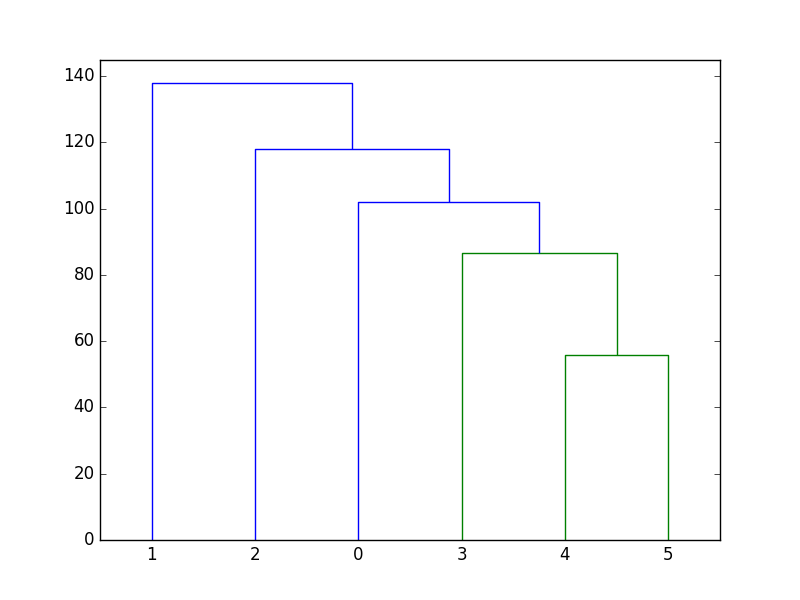
\includegraphics[width=5in]{\hierpath/figures/cluster6.png}}
\caption{Clusters of six data points.}
\label{fig:hierarchical:cluster6}
\end{figure}

This cluster is represented by the centroid $(\frac{15 + 66}{2},
\frac{20 + (-3)}{2}) = (\frac{81}{2}, \frac{17}{2}) = (40.5, 8.5)$.
The cluster is expressed as $(x_4, y_4)$ and $(x_5, y_5)$ is removed.
Now there are four data points and one cluster. The distances
are shown in Table~\ref{table:hierarchical:distance6points}.

\begin{table}
  \begin{tt}
\begin{tabular}{|r|rrrrr|}  \hline
& 0 & 1 & 2 & 3 & 4  \\ \hline

0 & 0& 42562& 14186& 10865 & 12674.5\\
1 & 42562& 0& 17096& 36445 & 11526.5 \\
2 & 14186& 17096& 0& 30617 & 11862.5 \\
3 & 10865& 36445& 30617& 0 & 7520.5 \\
4 & 12674.5 & 11526.5 & 11862.5 & 7520.5 & 0 \\  \hline
\end{tabular}
  \end{tt}
  \caption{Distances of pairs of six data points.}
  \label{table:hierarchical:distance6points}
\end{table}

The smallest distance is 7520.5 and it is between $(x_3, y_3)$ and the
cluster. Thus, $(x_3, y_3)$ and the cluster are put together by making
them the two childrens of a binary tree node.

To summarize, hierarchical cluster finds the closest pair of data
points, clusters, or one data point and one clusters and make them the
two children of a binary tree node.  The tree node because a new
cluster. This process continues until there is only cluster left.

\clearpage

Figures~\ref{fig:hierarchical:cluster2}-\ref{fig:hierarchical:cluster6}
are created using the following program.

\resetlinenumber[1]
\linenumbers
\begin{tt}
  \lstinputlisting{\progpath/unsupervised/hierarchical/examples/example1.py}
\end{tt}
\nolinenumbers

\section{Hierarchical Clustering Algorithm}

The hierarchical clustering algorithm starts by treating each data
point as a cluster. Then it repetively finds the closest two clusters.
These two clusters are the two children of a binary tree node and form
one cluster.  As a result, two clusters become one cluster.  This
process continues until only one cluster is left.
The algorithm is described below:

\begin{algorithm}
    \caption[]{Hierarchical Clustering Algorithm}
    \begin{algorithmic}[1]
      \ForAll  {data point}  make a cluster of its own
      \EndFor
      \While {Number of Cluster Exceeds one}
      \State Compute the distance of each pair of clusters
      \State Find the two clusters whose distance is the smallest
      \State Make these two clusters the children of a binary tree node
      \State Make this tree node a new cluster 
      \EndWhile
    \end{algorithmic}
    \label{algorithm:hierarchicalclustering}
\end{algorithm}

\section{Define Distance of Two Clusters}

\index{Cluster!Distance}

The earlier examples use the centroid to express each cluster.  Other
definitions of clusters' distances are also used.  There are four
commonly adopted definitions for the distance of two
clusters~\cite{James2013IntroductiontoStatistical}: {\it complete},
{\it single}, {\it average}, and {\it centroid}.  They are described
below.

Suppose $\mathds{A} = \{a_1, a_2, ..., a_n\}$ is a cluster
and $a_1$, $a_2$, ..., $a_n$ are the $n$ data points in this cluster.
Suppose $\mathds{B} = \{b_1, b_2, ..., b_m\}$ is another cluster
and $b_1$, $b_2$, ..., $b_m$ are the $m$ data points in this cluster.
The distance between these two clusters can be defined as

\begin{itemize}
\item Complete: Compute the pairwise distances of every point in
  $\mathds{A}$ and every point in $\mathds{B}$, then select the
  largest distance.  Mathematically, it is

  \begin{equation}
    \underset{a_i \in \mathds{A}, b_j \in \mathds{B}}{\max}
         {|a_i - b_j|}.
  \end{equation}

  Here, $|a_i - b_j|$ means the distance of the two points.

\item Single. This definition considers the smallest distance
  among all pairs of points in $\mathds{A}$ and $\mathds{B}$.
  
  \begin{equation}
    \underset{a_i \in \mathds{A}, b_j \in \mathds{B}}{\min}
         {|a_i - b_j|}.
  \end{equation}

\item Average. This definition computes the average of the pairwise
  distances.

  \begin{equation}
\frac{1}{n \times m}    \underset{a_i \in \mathds{A}, b_j \in \mathds{B}}{\Sigma}
         {|a_i - b_j|}.
  \end{equation}

\item Centroid. Find the centroid $c_{\mathds{A}}$ of $\mathds{A}$ and
  the centroid of $c_{\mathds{B}}$ $\mathds{B}$ using the definition
  of (\ref{equ:kmean:centroid}) in Chapter~\ref{chapter:kmean}.
  The distance of the two clusters is the distance of the two
  centroids:

  \begin{equation}
| c_{\mathds{A}} - c_{\mathds{B}} |.
    \end{equation}

  
\end{itemize}

\clearpage

% a good example in
% http://www.econ.upf.edu/~michael/stanford/maeb7.pdf


% how to plot tree: https://plot.ly/python/tree-plots/
% https://joernhees.de/blog/2015/08/26/scipy-hierarchical-clustering-and-dendrogram-tutorial/
